\section{Scale and Direction Generality Across the 65-Pair OMP Pool}
\label{app:attack_results}

The main text reports the 20-pair lightweight clique. This appendix completes the 65-pair OMP evaluation with the standard-scale clique ($\mathcal{C}_{\text{Std}}$) and the two cross-scale transfer suites ($\mathcal{T}_{\text{Cross}}^{\downarrow}$, $\mathcal{T}_{\text{Cross}}^{\uparrow}$). All values use the per-pair $\lambda$ from Appendix~\ref{app:lambda_sweep}; SER is measured on Alpaca, SQuAD v2, and GSM8K, and utility follows the main-text choices (\S\ref{subsec:exp-settings}).

\subsection{The Standard-Scale Clique ($\mathcal{C}_{\text{Std}}$)}

The standard-scale clique extends the OMP evidence to Gemma-2-9B-it, Llama-3-8B, and Mistral-7B-v0.1.
Figure~\ref{fig:app:large-bidirectional:ser-dumbbell} shows the SER asymmetry: across the 6 pairs, attacked-base $\mathrm{SER}_{\max}$ averages $0.54$ versus patched-donor $\mathrm{SER}_{\max}$ $0.043$ (${>}12\times$ gap), with Gem2-9B$\leftarrow$ML3-8B reaching attacked-base $\mathrm{SER}_{\max}=1.0000$ and donor $\mathrm{SER}_{\max}=.0039$.
Figure~\ref{fig:app:large-bidirectional:donor-util-id} shows donor-side utility on the identity line, and Figure~\ref{fig:app:large-bidirectional:base-util-slope} shows the base-side three-stage trajectory (pretrained $\to$ after-OMP $\to$ after-attack).

\begin{figure}[t]
  \centering
  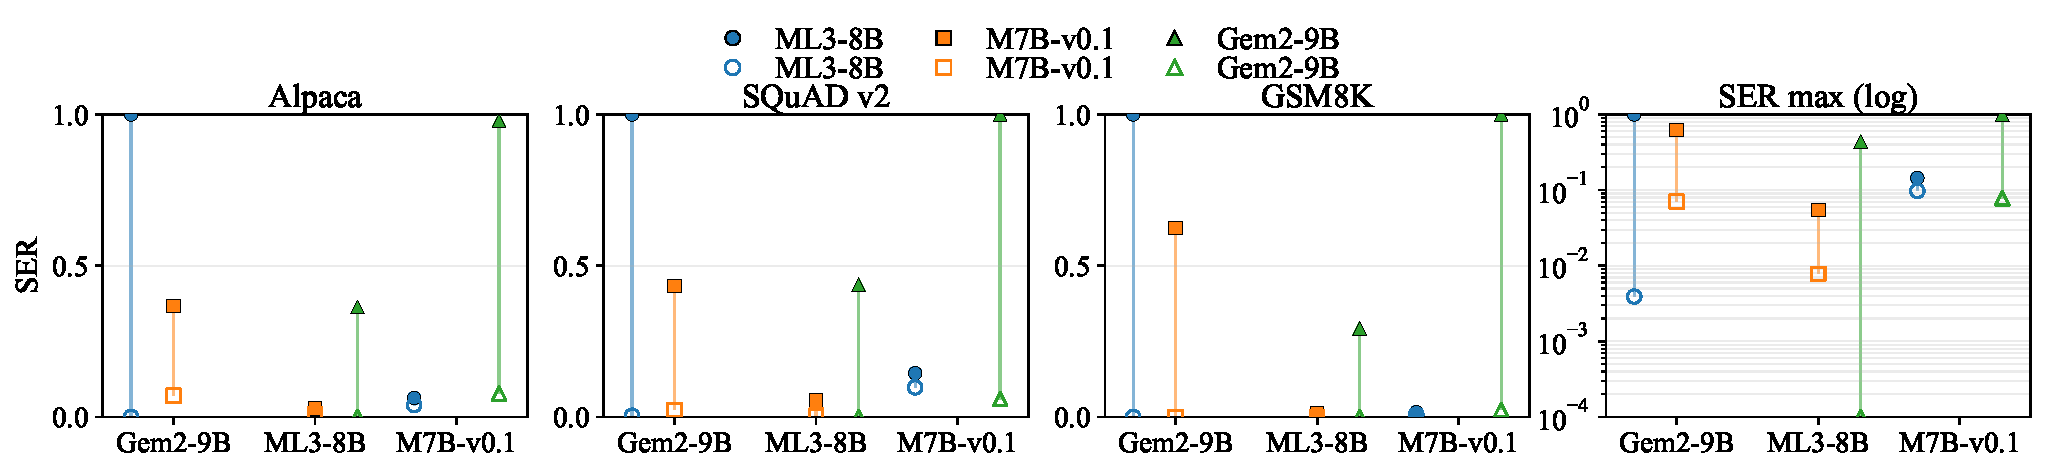
\includegraphics[width=\linewidth]{paper/figures/app_large_bidirectional_ser_dumbbell_grid.pdf}
  \vspace{-6mm}
  \caption{The standard-scale clique preserves the same SER asymmetry as the lightweight clique. Columns show Alpaca, SQuAD v2, GSM8K, and $\mathrm{SER}_{\max}$; each dumbbell connects patched-donor SER (open) to attacked-base SER (filled).}
  \label{fig:app:large-bidirectional:ser-dumbbell}
\end{figure}
\begin{figure}[t]
  \centering
  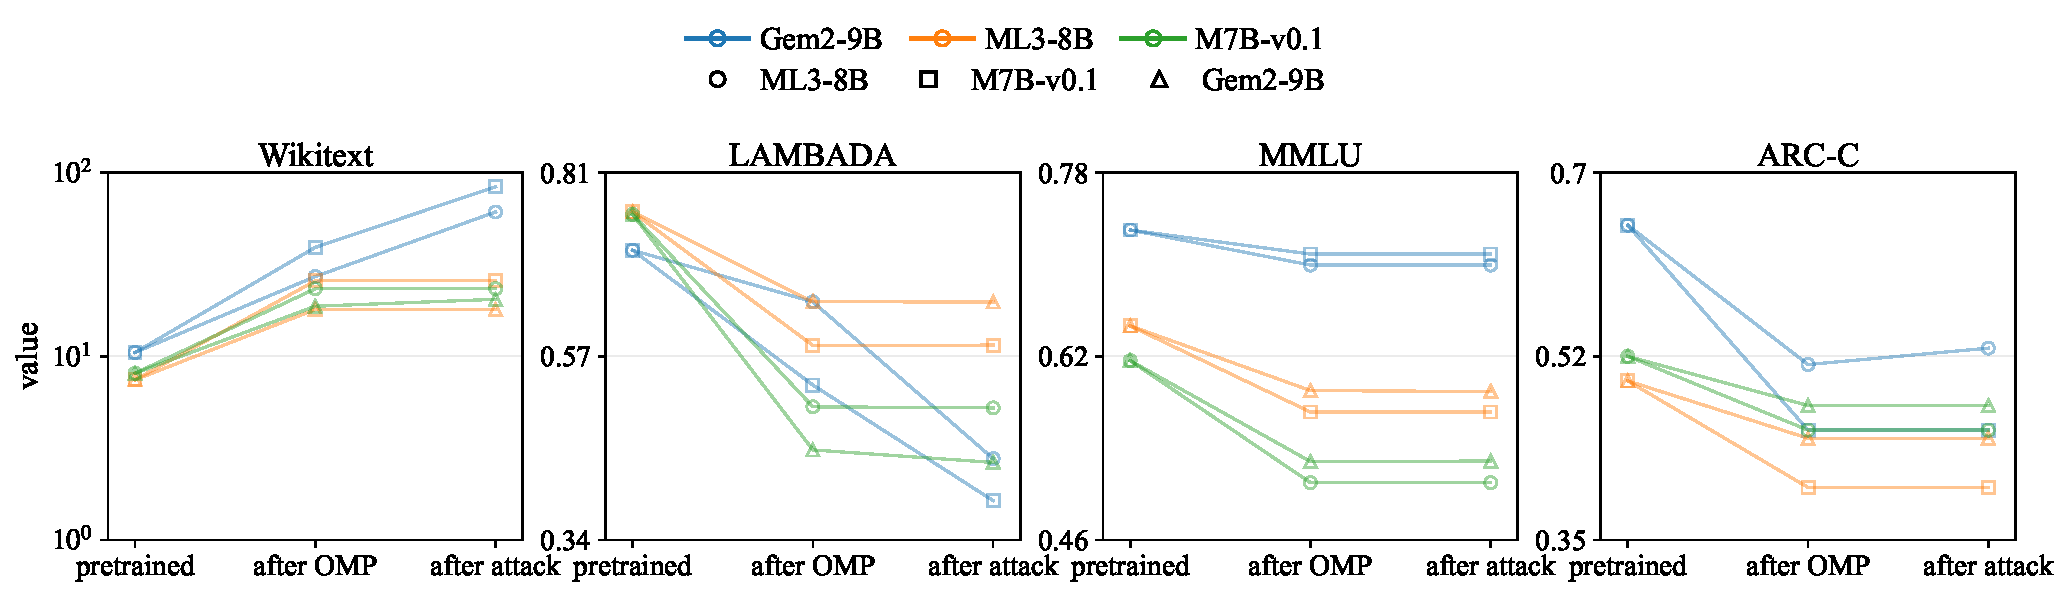
\includegraphics[width=\linewidth]{paper/figures/app_large_bidirectional_base_utility_slope_3stage_grid.pdf}
  \vspace{-6mm}
  \caption{Standard-scale base utility follows the same pretrained $\to$ after-OMP $\to$ after-attack trajectory as in the main text. Each line is one pair (base$\leftarrow$donor).}
  \label{fig:app:large-bidirectional:base-util-slope}
\end{figure}
\begin{figure}[t]
  \centering
  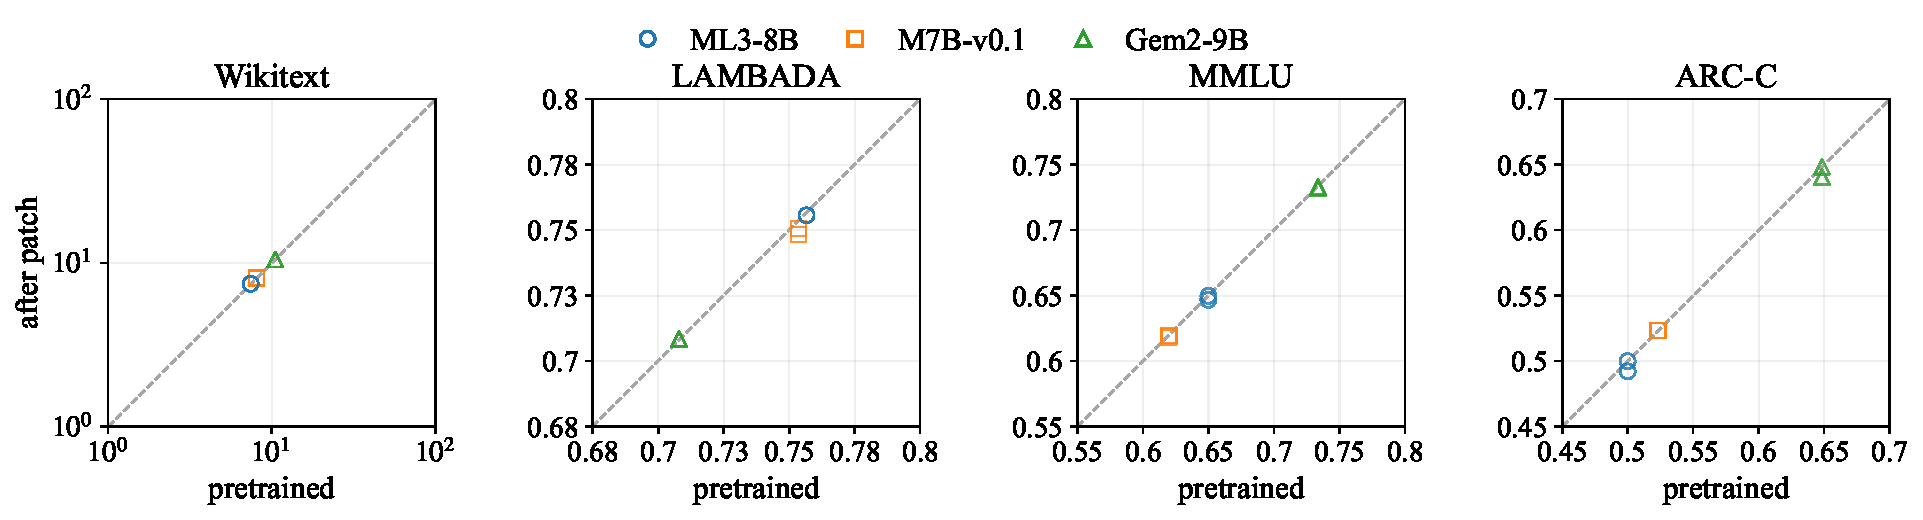
\includegraphics[width=\linewidth]{paper/figures/app_large_bidirectional_donor_utility_identity_scatter_grid.pdf}
  \vspace{-6mm}
  \caption{Standard-scale donor utility remains close to the identity line after patching. Each point is one pair; x-axis is donor pretrained utility and y-axis is post-patch utility.}
  \label{fig:app:large-bidirectional:donor-util-id}
\end{figure}

\subsection{Cross-Scale Transfer Sets ($\mathcal{T}_{\text{Cross}}^{\downarrow}$), downstream (small base$\leftarrow$large donor)}

Downstream transfer covers small bases (SmolLM2, Qwen2.5, Gemma-2/3, Llama-3.2) receiving rows from large donors (Qwen2/3, Llama-3, Mistral-7B).
Figure~\ref{fig:app:small-to-large-oneperfamily:ser-dumbbell} shows median attacked-base $\mathrm{SER}_{\max}=0.9336$ with 12/23 pairs at $\mathrm{SER}_{\max}\ge0.9$ and donor $\mathrm{SER}_{\max}\le0.01$; representative pairs (Gem2-2B$\leftarrow$ML3-8B, Gem2-2B$\leftarrow$L3.1-8B) reach attacked-base $\mathrm{SER}_{\max}=1.0000$ with donor $\mathrm{SER}_{\max}=0.0000$.
Figure~\ref{fig:app:small-to-large-oneperfamily:donor-util-id} shows donor-side identity-line stability, and Figure~\ref{fig:app:small-to-large-oneperfamily:base-util-slope} shows the base three-stage trajectory.

\begin{figure}[t]
  \centering
  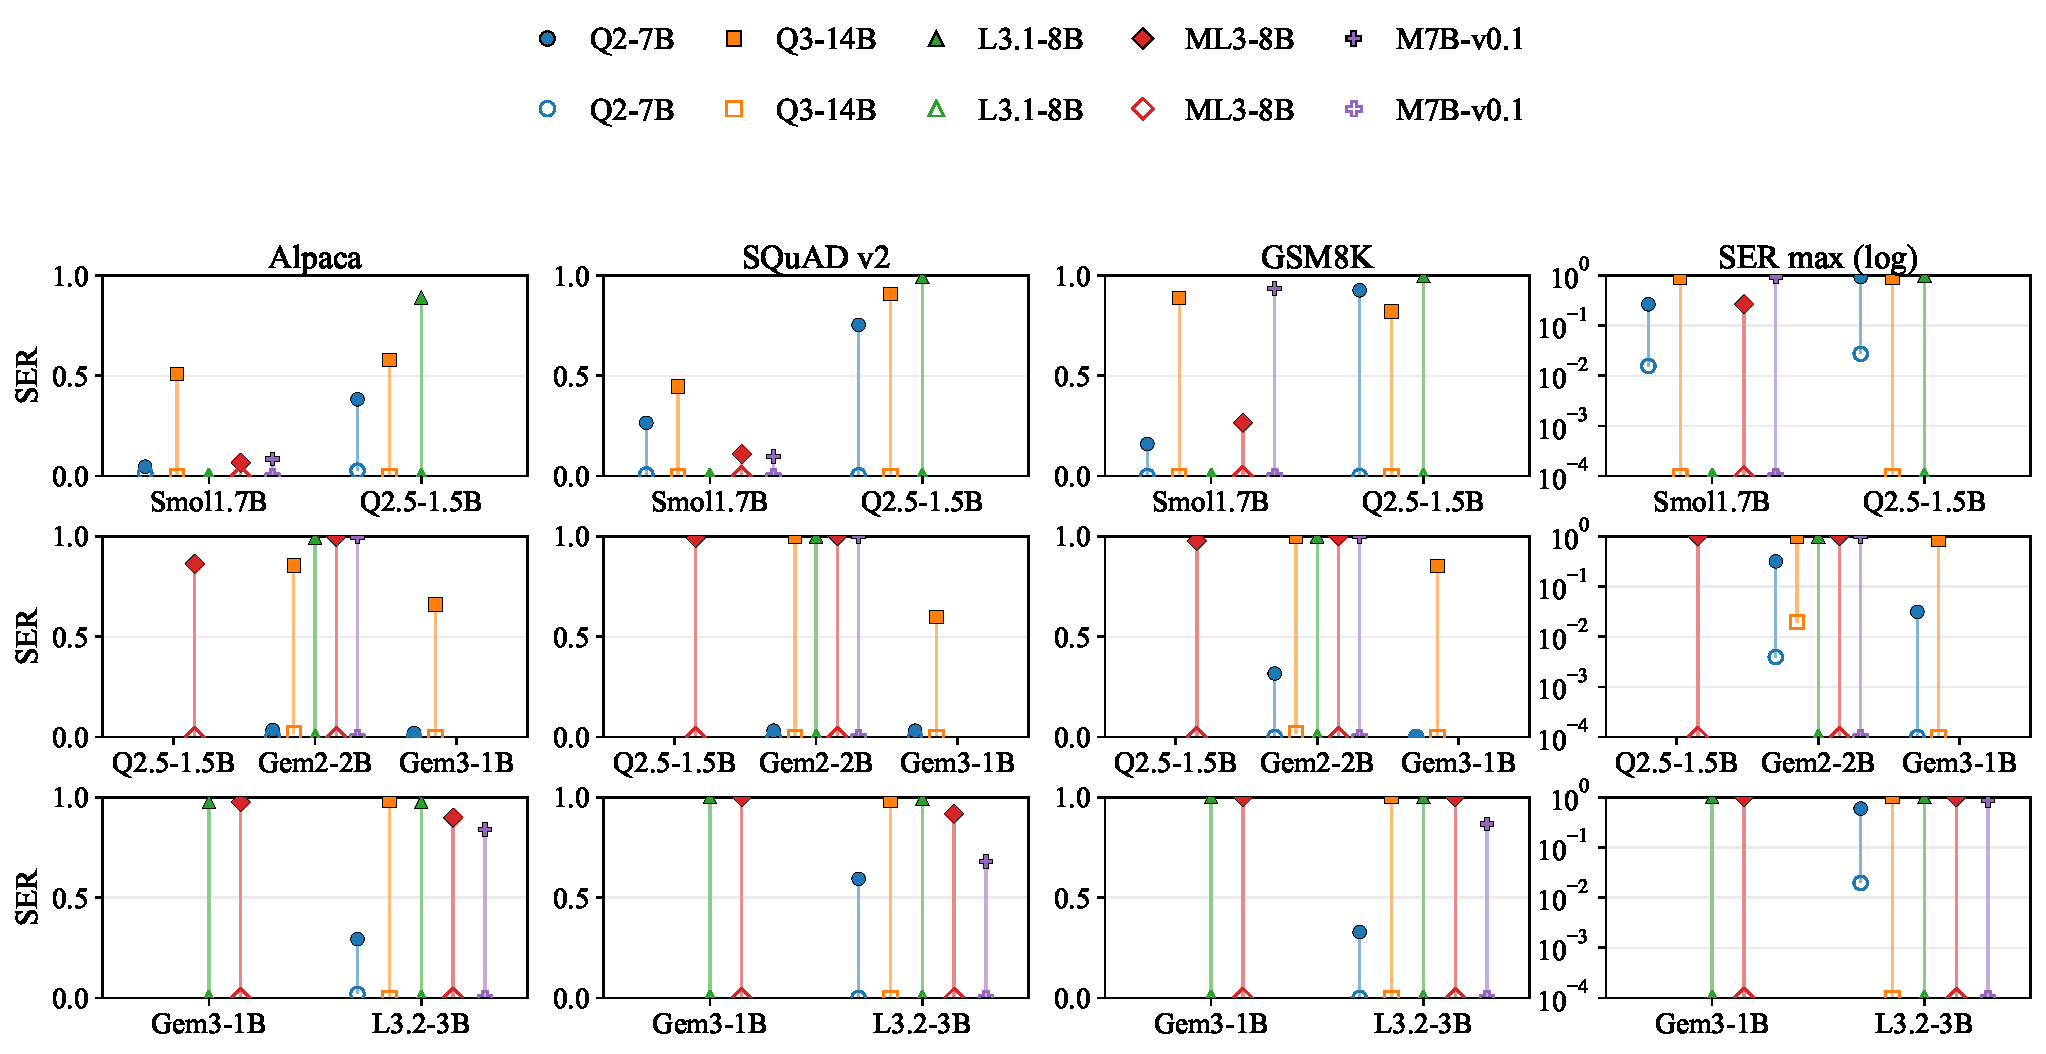
\includegraphics[width=\linewidth]{paper/figures/app_small_to_large_oneperfamily_ser_dumbbell_grid.pdf}
  \vspace{-6mm}
  \caption{Downstream cross-scale transfer reaches high attacked-base SER with donor SER near zero. Each dumbbell connects patched-donor SER (open) to attacked-base SER (filled).}
  \label{fig:app:small-to-large-oneperfamily:ser-dumbbell}
\end{figure}
\begin{figure}[t]
  \centering
  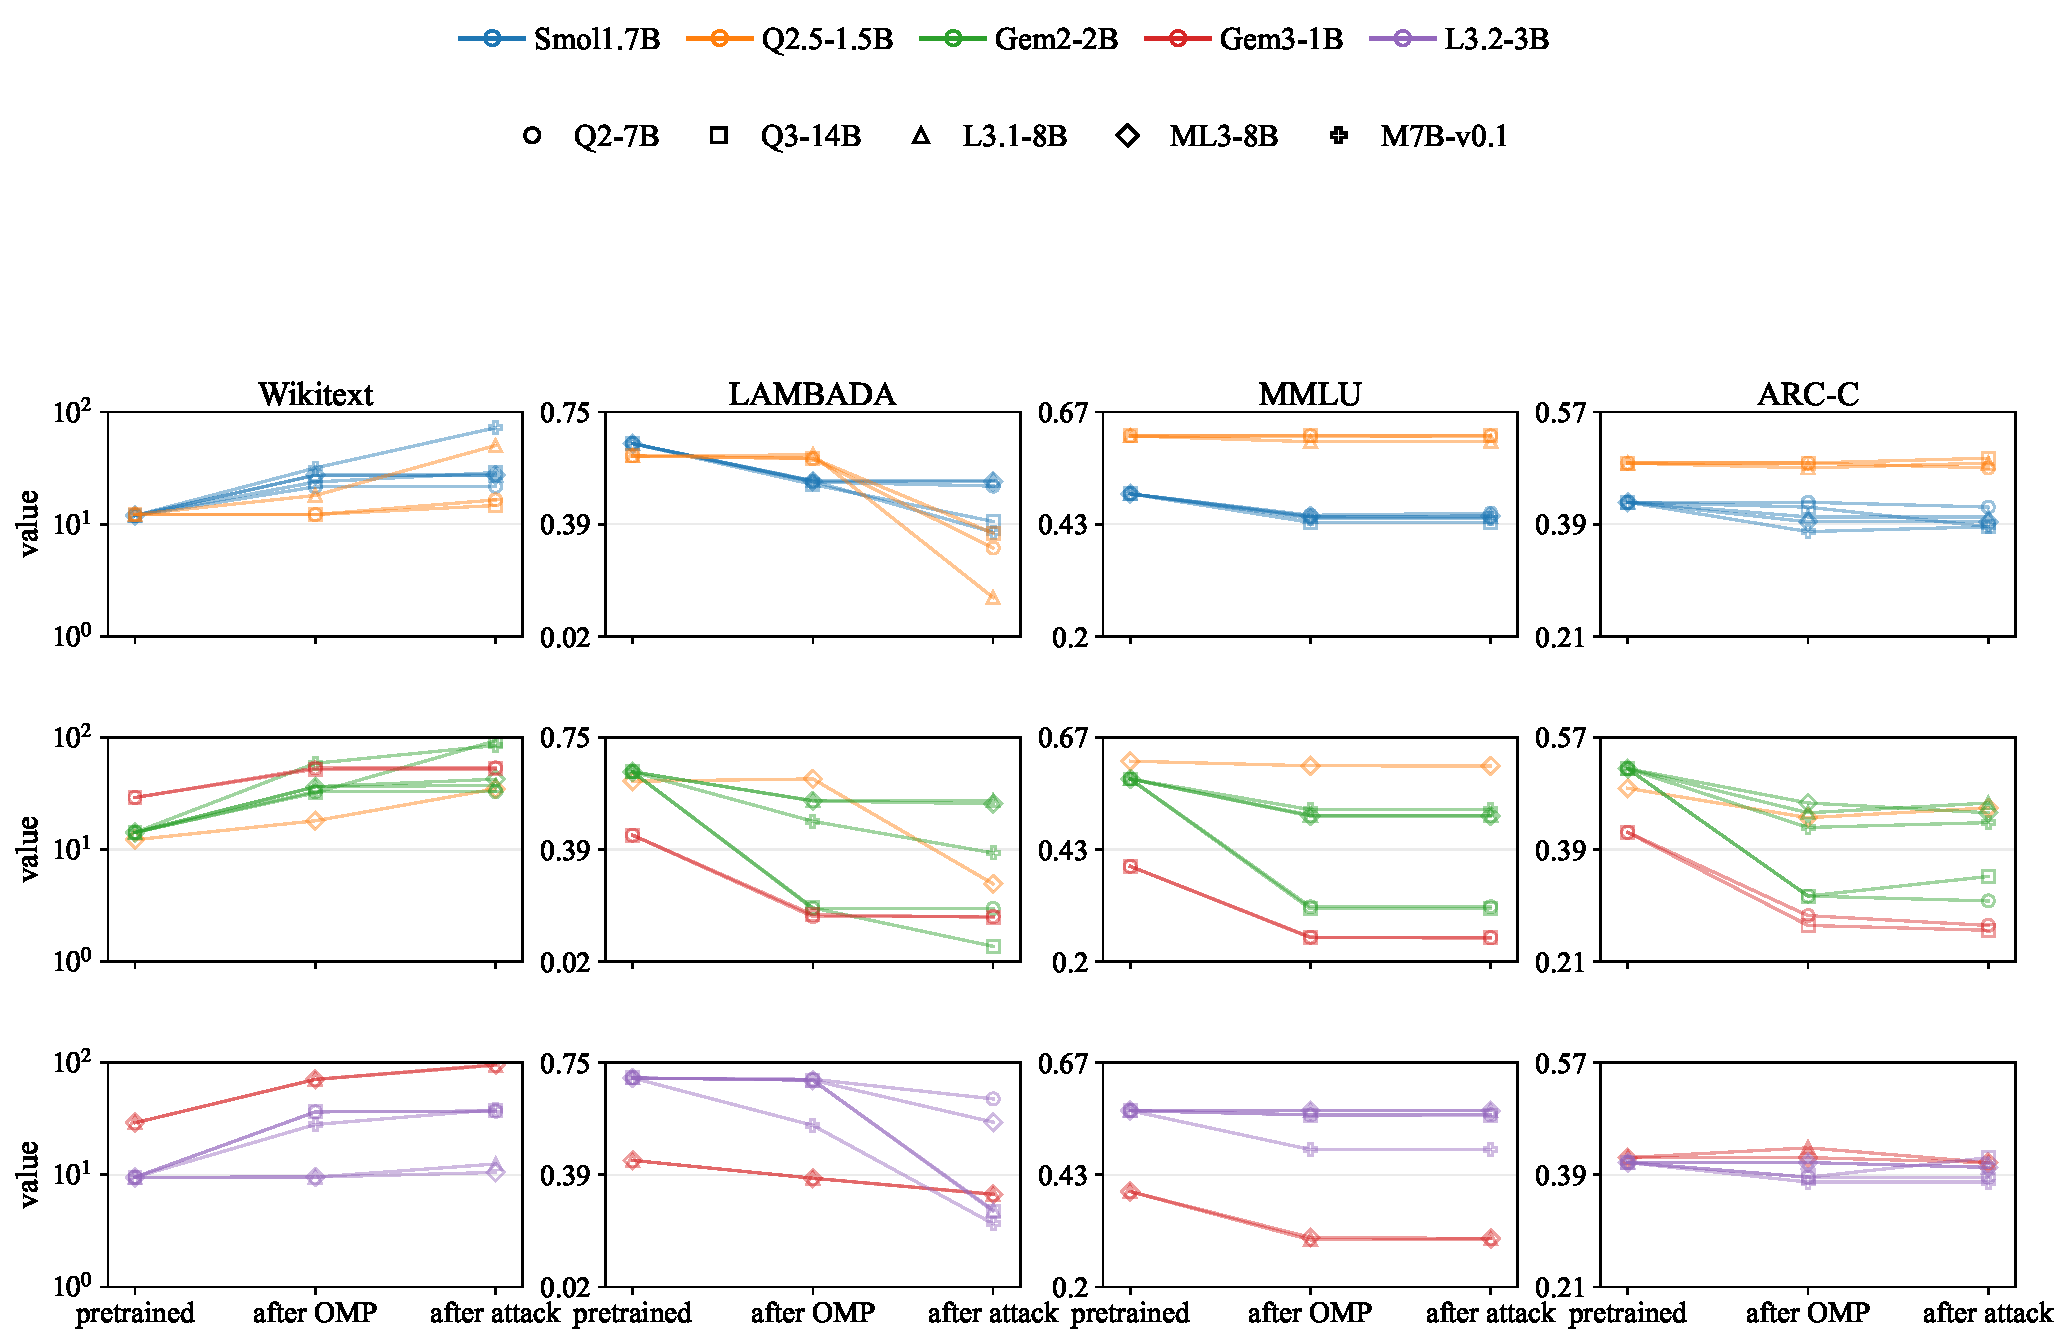
\includegraphics[width=\linewidth]{paper/figures/app_small_to_large_oneperfamily_base_utility_slope_3stage_grid.pdf}
  \vspace{-6mm}
  \caption{Downstream base-utility trajectories show the pretrained $\to$ after-OMP $\to$ after-attack path for small bases receiving rows from large donors.}
  \label{fig:app:small-to-large-oneperfamily:base-util-slope}
\end{figure}
\begin{figure}[t]
  \centering
  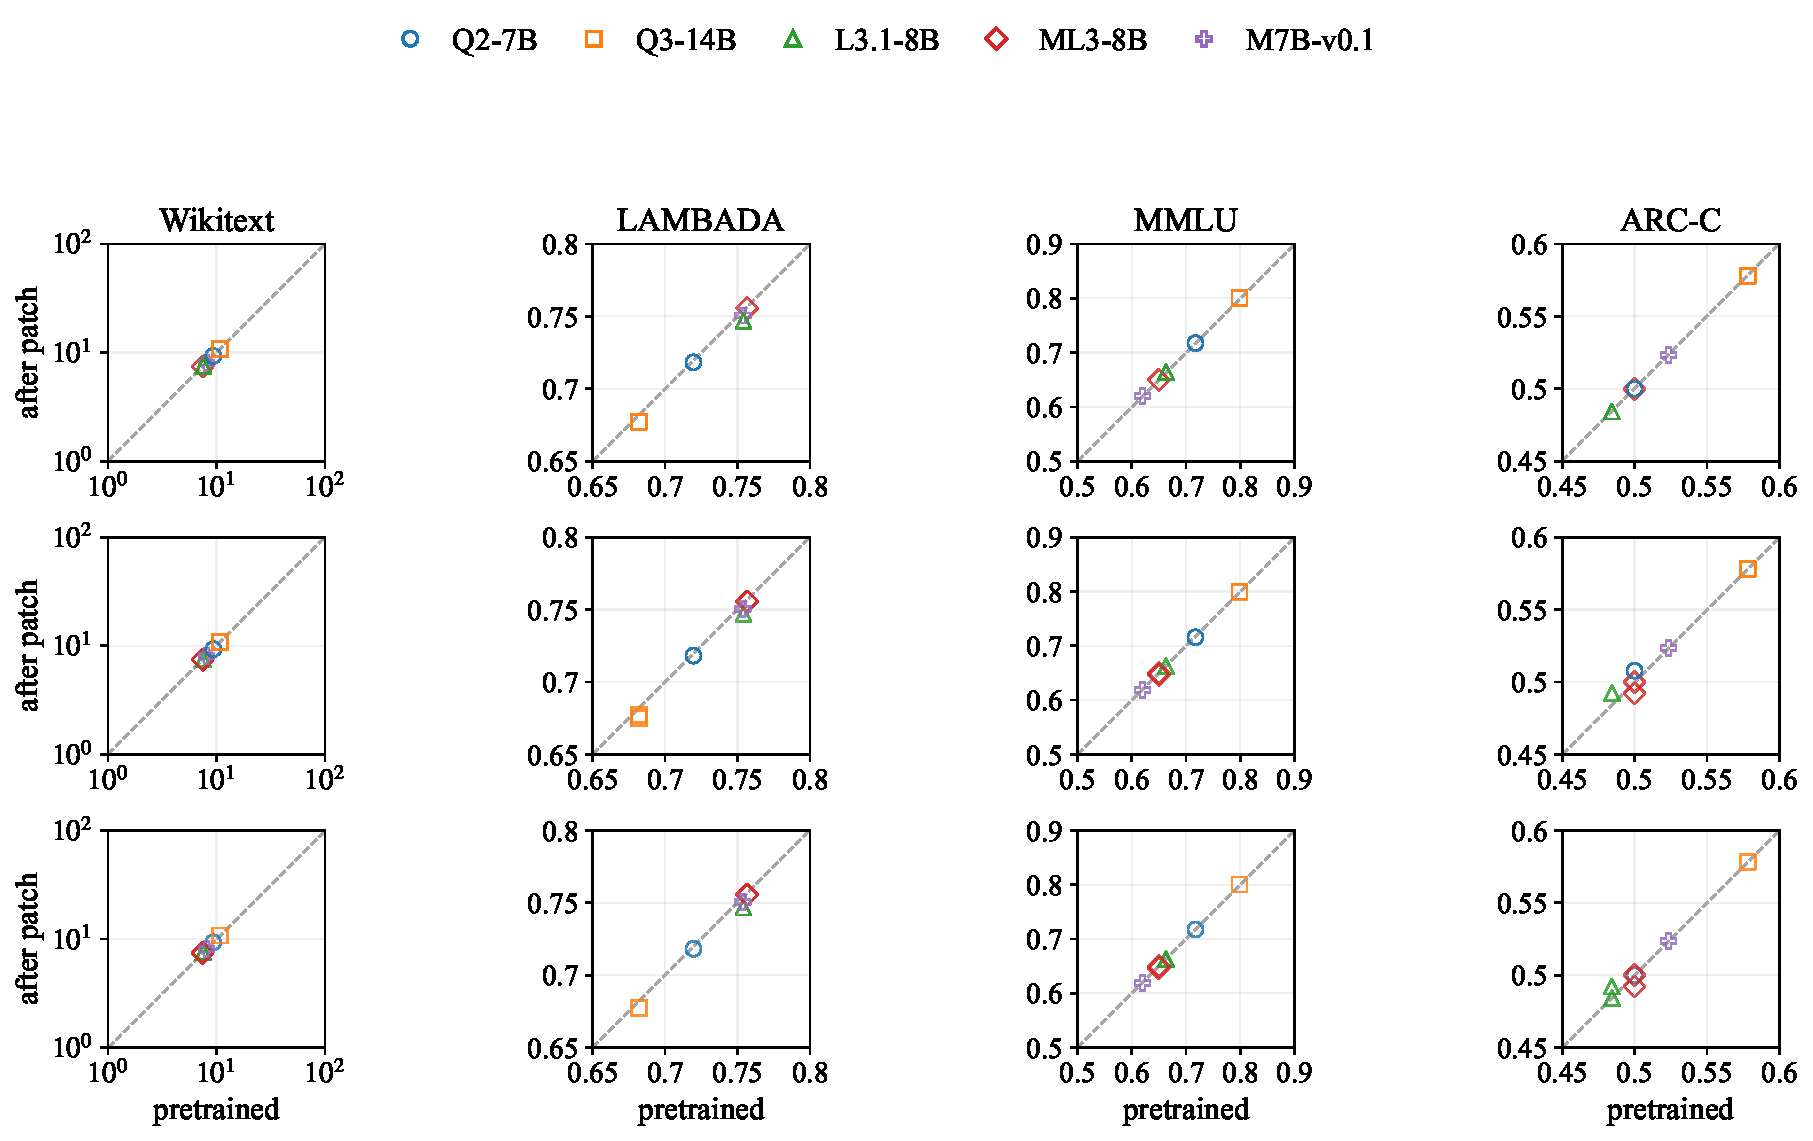
\includegraphics[width=\linewidth]{paper/figures/app_small_to_large_oneperfamily_donor_utility_identity_scatter_grid.pdf}
  \vspace{-6mm}
  \caption{Downstream donor utility remains stable after patching for the small-base, large-donor transfer suite.}
  \label{fig:app:small-to-large-oneperfamily:donor-util-id}
\end{figure}

\subsection{Cross-Scale Transfer Sets ($\mathcal{T}_{\text{Cross}}^{\uparrow}$), upstream (large base$\leftarrow$small donor)}

Upstream transfer covers large bases (Qwen2-7B, Llama-3, Mistral-7B) receiving rows from small donors (Qwen3-0.6B, Gemma-2/3, Ministral-3B).
Figure~\ref{fig:app:large-to-small-oneperfamily:ser-dumbbell} shows the SER asymmetry: across 16 pairs, attacked-base $\mathrm{SER}_{\max}$ averages $0.65$ versus donor $\mathrm{SER}_{\max}$ average $0.078$ (median donor $.0117$), with strong pairs such as ML3-8B$\leftarrow$Gem2-2B reaching attacked-base $\mathrm{SER}_{\max}=1.0000$ and donor $.0039$.
Figure~\ref{fig:app:large-to-small-oneperfamily:donor-util-id} shows donor-side utility, and Figure~\ref{fig:app:large-to-small-oneperfamily:base-util-slope} shows the base three-stage trajectory.

\begin{figure}[t]
  \centering
  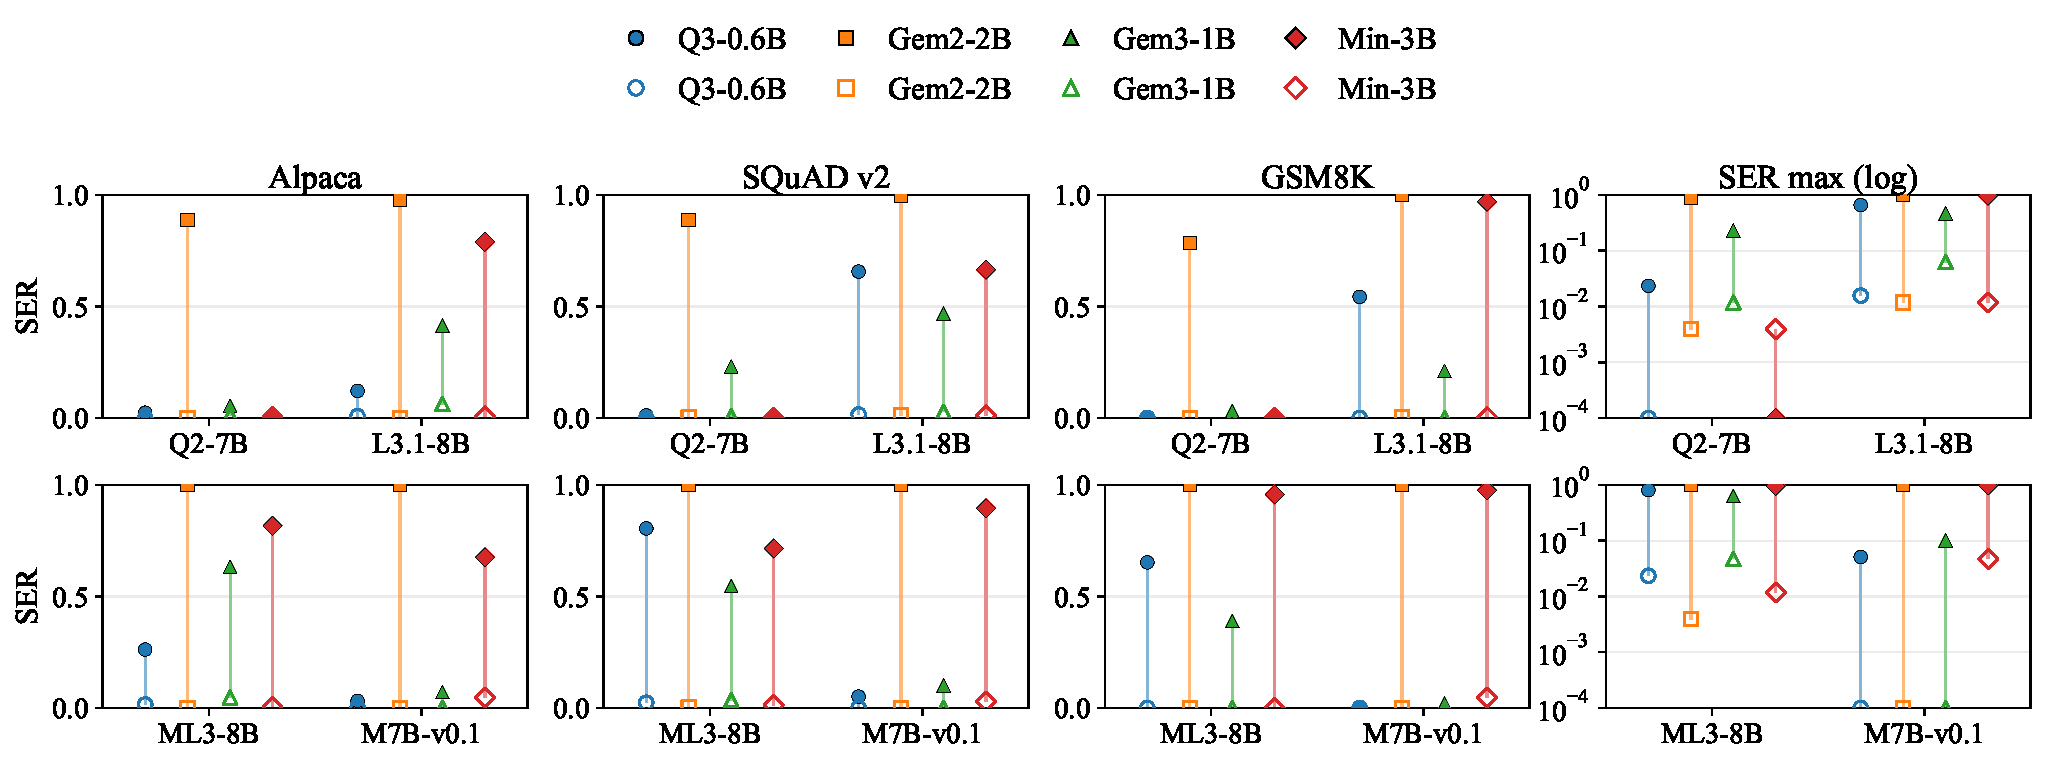
\includegraphics[width=\linewidth]{paper/figures/app_large_to_small_oneperfamily_ser_dumbbell_grid.pdf}
  \vspace{-6mm}
  \caption{Upstream cross-scale transfer preserves the attacked-base versus donor SER gap across 16 large-base, small-donor pairs. Each dumbbell connects patched-donor SER (open) to attacked-base SER (filled).}
  \label{fig:app:large-to-small-oneperfamily:ser-dumbbell}
\end{figure}
\begin{figure}[t]
  \centering
  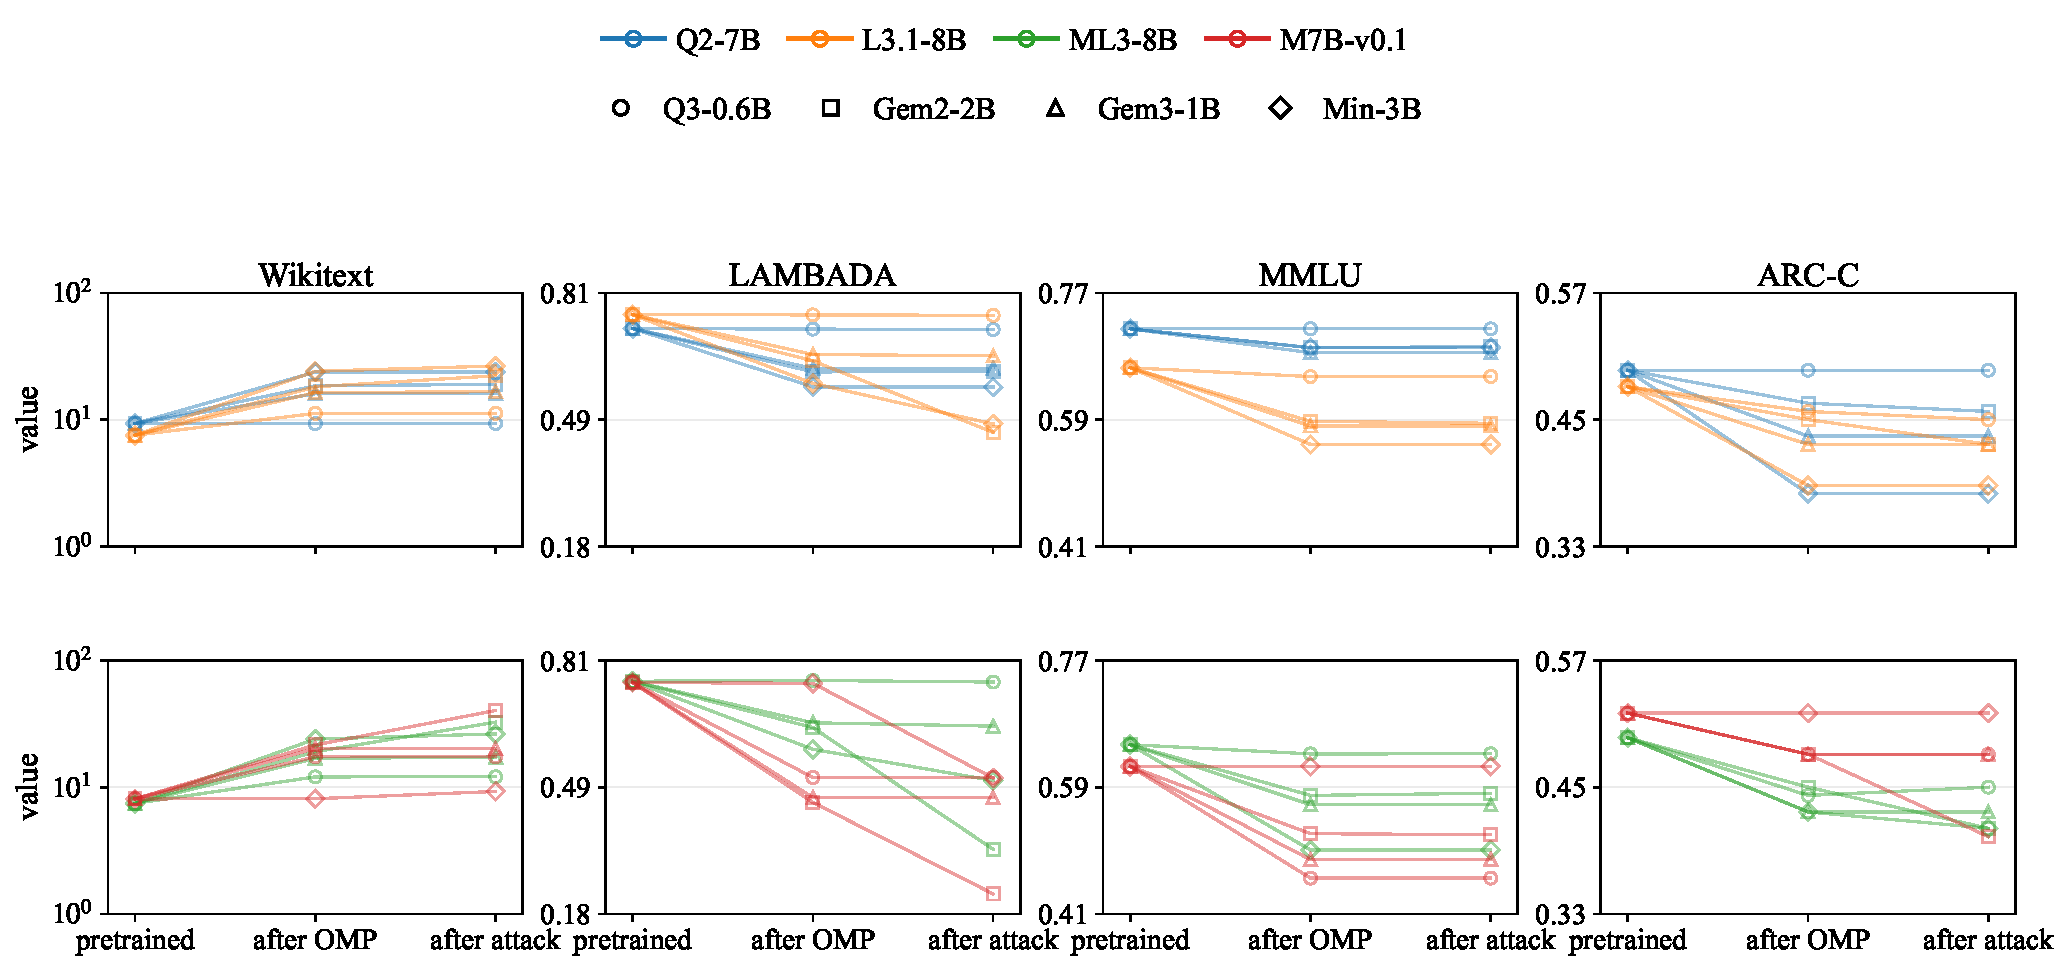
\includegraphics[width=\linewidth]{paper/figures/app_large_to_small_oneperfamily_base_utility_slope_3stage_grid.pdf}
  \vspace{-6mm}
  \caption{Upstream base-utility trajectories track the pretrained $\to$ after-OMP $\to$ after-attack path for large bases receiving rows from small donors.}
  \label{fig:app:large-to-small-oneperfamily:base-util-slope}
\end{figure}
\begin{figure}[t]
  \centering
  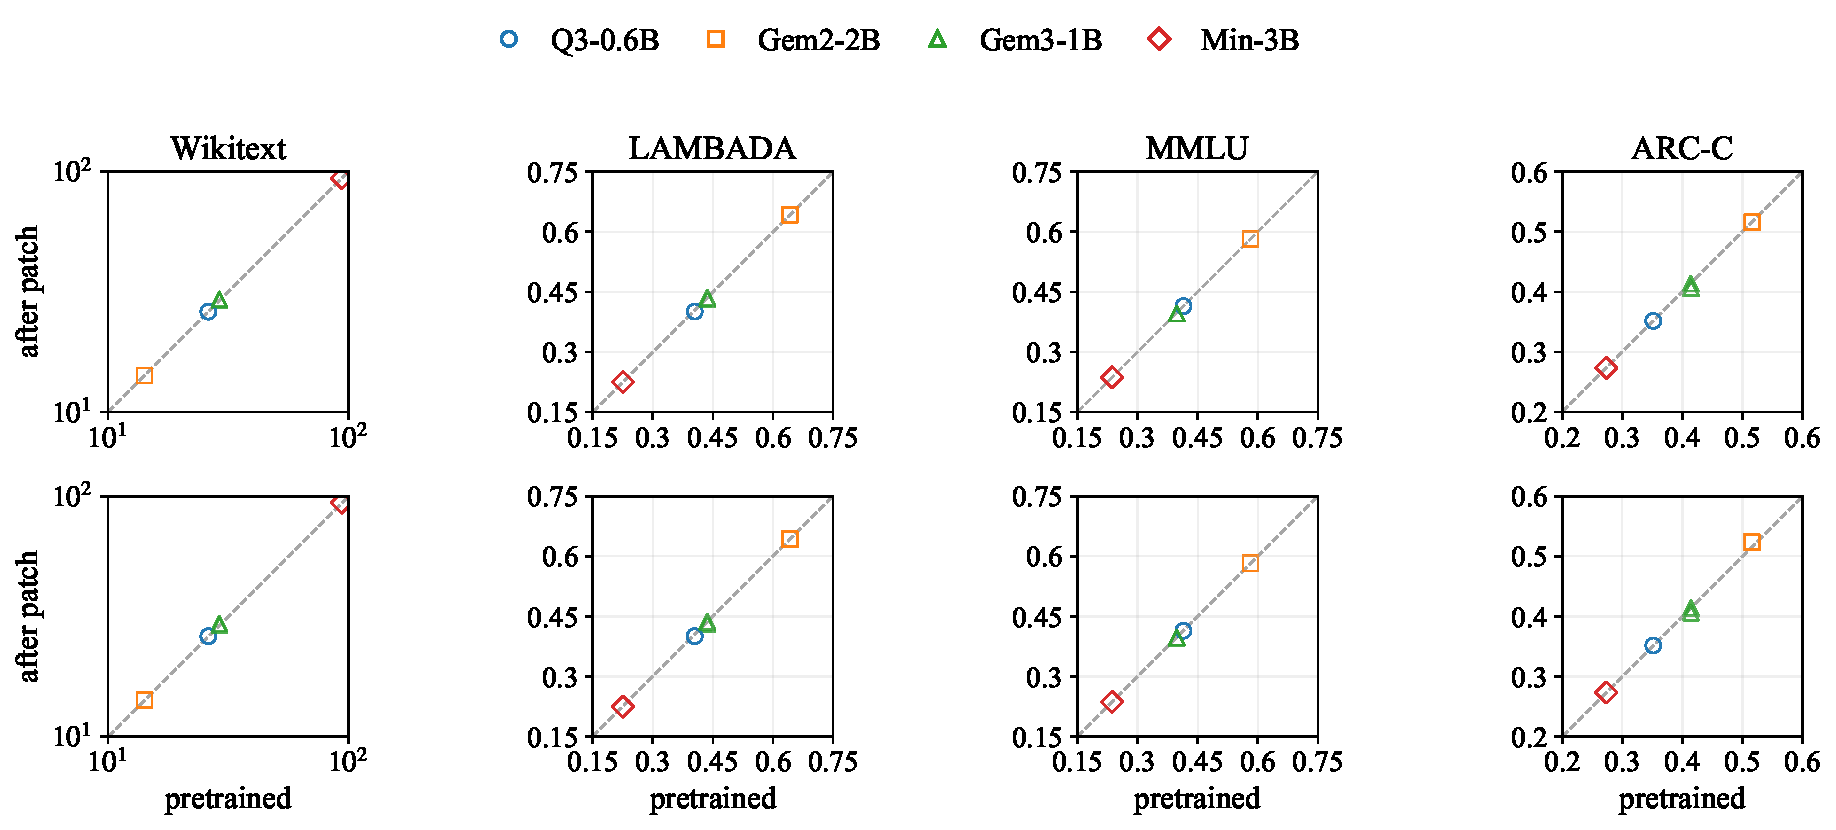
\includegraphics[width=\linewidth]{paper/figures/app_large_to_small_oneperfamily_donor_utility_identity_scatter_grid.pdf}
  \vspace{-6mm}
  \caption{Upstream donor utility remains stable after patching for the large-base, small-donor transfer suite.}
  \label{fig:app:large-to-small-oneperfamily:donor-util-id}
\end{figure}
